% ============================================================
%  Figure — r1 ratio ablation
%  Required preamble packages:
%    \usepackage{graphicx}
% ============================================================

\begin{figure*}[t]
\centering
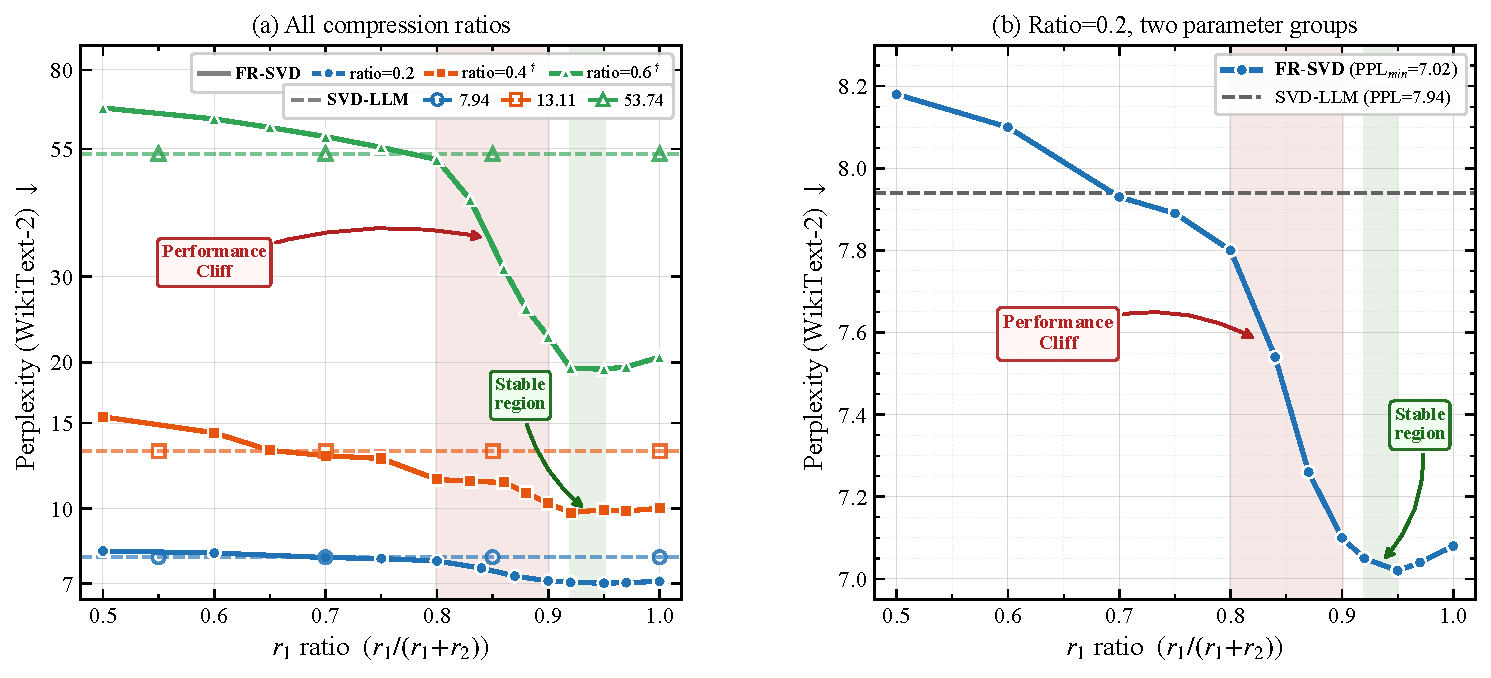
\includegraphics[width=0.8\textwidth]{figs/r1_ratio_ablation.pdf}
\caption{Ablation on rank budget allocation ($r_1$ ratio $= r_1/(r_1+r_2)$) across three
compression ratios on LLaMA-7B (WikiText-2 perplexity, lower is better).
\textbf{(a)} Overview across all compression ratios; SVD-LLM baselines are shown as
horizontal dashed lines. \textbf{(b)} Zoom-in at ratio\,=\,0.2 to visualize the
cliff--plateau transition near the optimum. Coefficient-selection settings are
specified in Appendix~\ref{app:rank-allocation}.
Both subplots reveal two characteristic regions: a \emph{Performance Cliff}
($r_1/r\!\approx\!0.80$--$0.90$) where PPL drops rapidly as more rank is allocated to
Stage~1, and a \emph{Stable Region} ($r_1/r\!\approx\!0.92$--$0.95$) where PPL reaches its
minimum plateau. Setting $r_1/r=1$ (no Stage-2 compensation) causes PPL to rise slightly,
confirming the benefit of reserving a small rank budget for residual compensation.}
\label{fig:r1-ablation}
\end{figure*}
